\documentclass[a4paper, 11pt]{article}
\usepackage[ngerman]{babel}
%ä und so
\usepackage[utf8]{inputenc}
\usepackage[T1]{fontenc}
\usepackage{amsmath}
\usepackage{amsthm}
\usepackage{amsbsy}

\usepackage{mathrsfs}
\usepackage{amssymb}
\usepackage{amstext}
\usepackage{amsfonts}
\usepackage{float}
\usepackage{graphicx}
\usepackage{esdiff}
\usepackage{hyperref}
\usepackage{geometry}
\geometry{top = 20mm, bottom = 20 mm, left = 25mm, right = 25mm}


\usepackage{setspace}
\onehalfspacing

\usepackage{fancyhdr}
\usepackage{wrapfig}
%\usepackage[hyphens]{url}
%\urlstyle{sf}
%\usepackage[hidelinks]{hyperref}
%\usepackage{breakurl}
%\hypersetup{colorlinks=false}
\usepackage{multirow}
\usepackage[bottom]{footmisc}
\usepackage{makecell}

%\usepackage{svg}

\title{Wärmelehre: \\ Bestimmung des Adiabatenkoeffizienten $\kappa = c_p / c_v$}
\author{Gruppe 2 \\ \\ Adelind Elshani \\ Olexiy Fedorets}
\date{\today}

% !TeX spellcheck = de_DE
\begin{document}


\begin{titlepage}
	\vspace*{\fill}
	\begin{center}
		\vskip -0.25\textheight
		\vfill
		\newcommand{\Line}{\rule{\linewidth}{0.6mm}}
		\Line 
		{\let\newpage\relax\maketitle}
		\Line 
		\vfill
	\end{center}
	\vspace*{\fill}
	\thispagestyle{empty}
\end{titlepage}





\newpage
\thispagestyle{empty}
\tableofcontents
\newpage

%Kopf- und Fußzeile
\pagestyle{fancy}
\fancyhf{}
%Kopfzeile links bzw. innen
\fancyhead[L]{\nouppercase{\leftmark}}
%Kopfzeile rechts bzw. außen
\fancyhead[R]{\thepage}
%Linie oben
\renewcommand{\headrulewidth}{0.5pt}
\fancyfoot[C]{\thepage}


\setcounter{page}{1}

\section{Einleitung}
In diesem Versuch soll der Adiabatenkoeffizient, also das Verhältnis $C_p/C_V$ mit der Methode nach Rüchardt bestimmt werden.

\section{Grundlagen}
Eine in einem Rohr befindliche Stahlkugel befindet sich genau dann im Gleichgewicht, wenn gilt
\begin{equation}
p = p_0 + \frac{mg}{A}.
\end{equation}
Wird die Kugel aus seiner Gleichgewichtsposition um die Strecke $x$ ausgelenkt, so ändert sich der Druck. Es wirkt daher die Kraft $Adp$ und die Reibungskraft $F_{fr} = -\alpha_{fr} \cdot \frac{dx}{dt}$ auf die Kugel. Dieser Prozess kann als quasi adiabatisch angesehen werden, es gilt daher $pV^{\kappa} = const$. Mit 
\begin{equation}
dp = -\frac{p\kappa}{V} dV
\end{equation}
und
\begin{equation}
dV = A \cdot x
\end{equation}
erhält man die Differentialgleichung 
\begin{equation}
\frac{d^2x}{dt^2} + \frac{\alpha_{fr}}{m} \cdot \frac{dx}{dt} + \frac{p \kappa A^2}{mV} \cdot x = 0.
\end{equation}
Dies ist die Differentialgleichung einer gedämpften harmonischen Schwingung mit der Eigenfrequenz
\begin{equation}
\omega_0 = \sqrt{\frac{p \kappa A^2}{mV}}
\end{equation}
Da eine gedämpfte Schwingung vorliegt setzt sich die Frequenz aus der Eigenfrequenz und der Dämpfung zusammen:
\begin{equation}\label{eq:omega}
\omega^2 = \omega_0^2 - \delta^2
\end{equation}
Daraus erhält man den Adiabatenkoeffizienten: 
\begin{equation}
\kappa = \omega_0^2 \frac{mV}{pA^2}
\end{equation}


\clearpage
\section{Aufbau und Durchführung}
Der Aufbau ist in der Abbildung \ref{fig:Aufbau des Versuchs} dargestellt. Ein Glasrohr wird in eine Mariottsche Flasche gesteckt und mit einem Gummiring luftdicht abgedichtet. An der Seite ist eine weitere Öffnung, durch die einmal ein Luftstrom, mithilfe einer Handpumpe, erzeugt werden kann und zum anderen der Druck, mithilfe eines Differenzialdrucksensors, gemessen werden kann.

\noindent
Eine Stahlkugel wird nun in die obere Öffnung eingeführt und, mittels der Handpumpe, zum schweben gebracht. Wird die Kugel nun schnell mit zwei Permanentmagneten nach oben bewegt, so fängt die Kugel an zu schwingen. Vor der Auslenkung wird die gewünschte Gleichgewichtslage markiert. Anschließend wartet man nach dem Druckaufbau, bis die Kugel die Markierung erreicht hat und lenkt sie in diesem Moment aus. Dadurch ist eine genauere Messung möglich. 

Mit dem Cassy-Modul wird der Druck in der Flasche während der Schwingung aufgezeichnet, und daraus die Kreisfrequenz der Schwingung bestimmt. Es werden Messungen an unterschiedlichen Postionen im Rohr durchgeführt. Der Messbereich des Drucksensors liegt bei $\pm 21 hPa$ und es werden bei einem Messintervall von einer halben Millisekunde 8000 Messungen durchgeführt, was einer Messzeit von 4s entspricht.
\begin{figure}[H]
	\begin{minipage}[t]{0.45\linewidth}
		\centering
		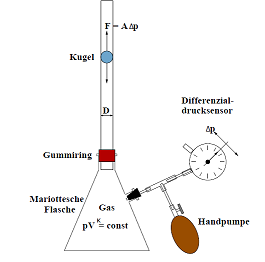
\includegraphics[scale=1]{Aufbau.png}
	\end{minipage}
	\hspace{0.05\linewidth}
	\begin{minipage}[t]{0.45\linewidth}
		\centering
		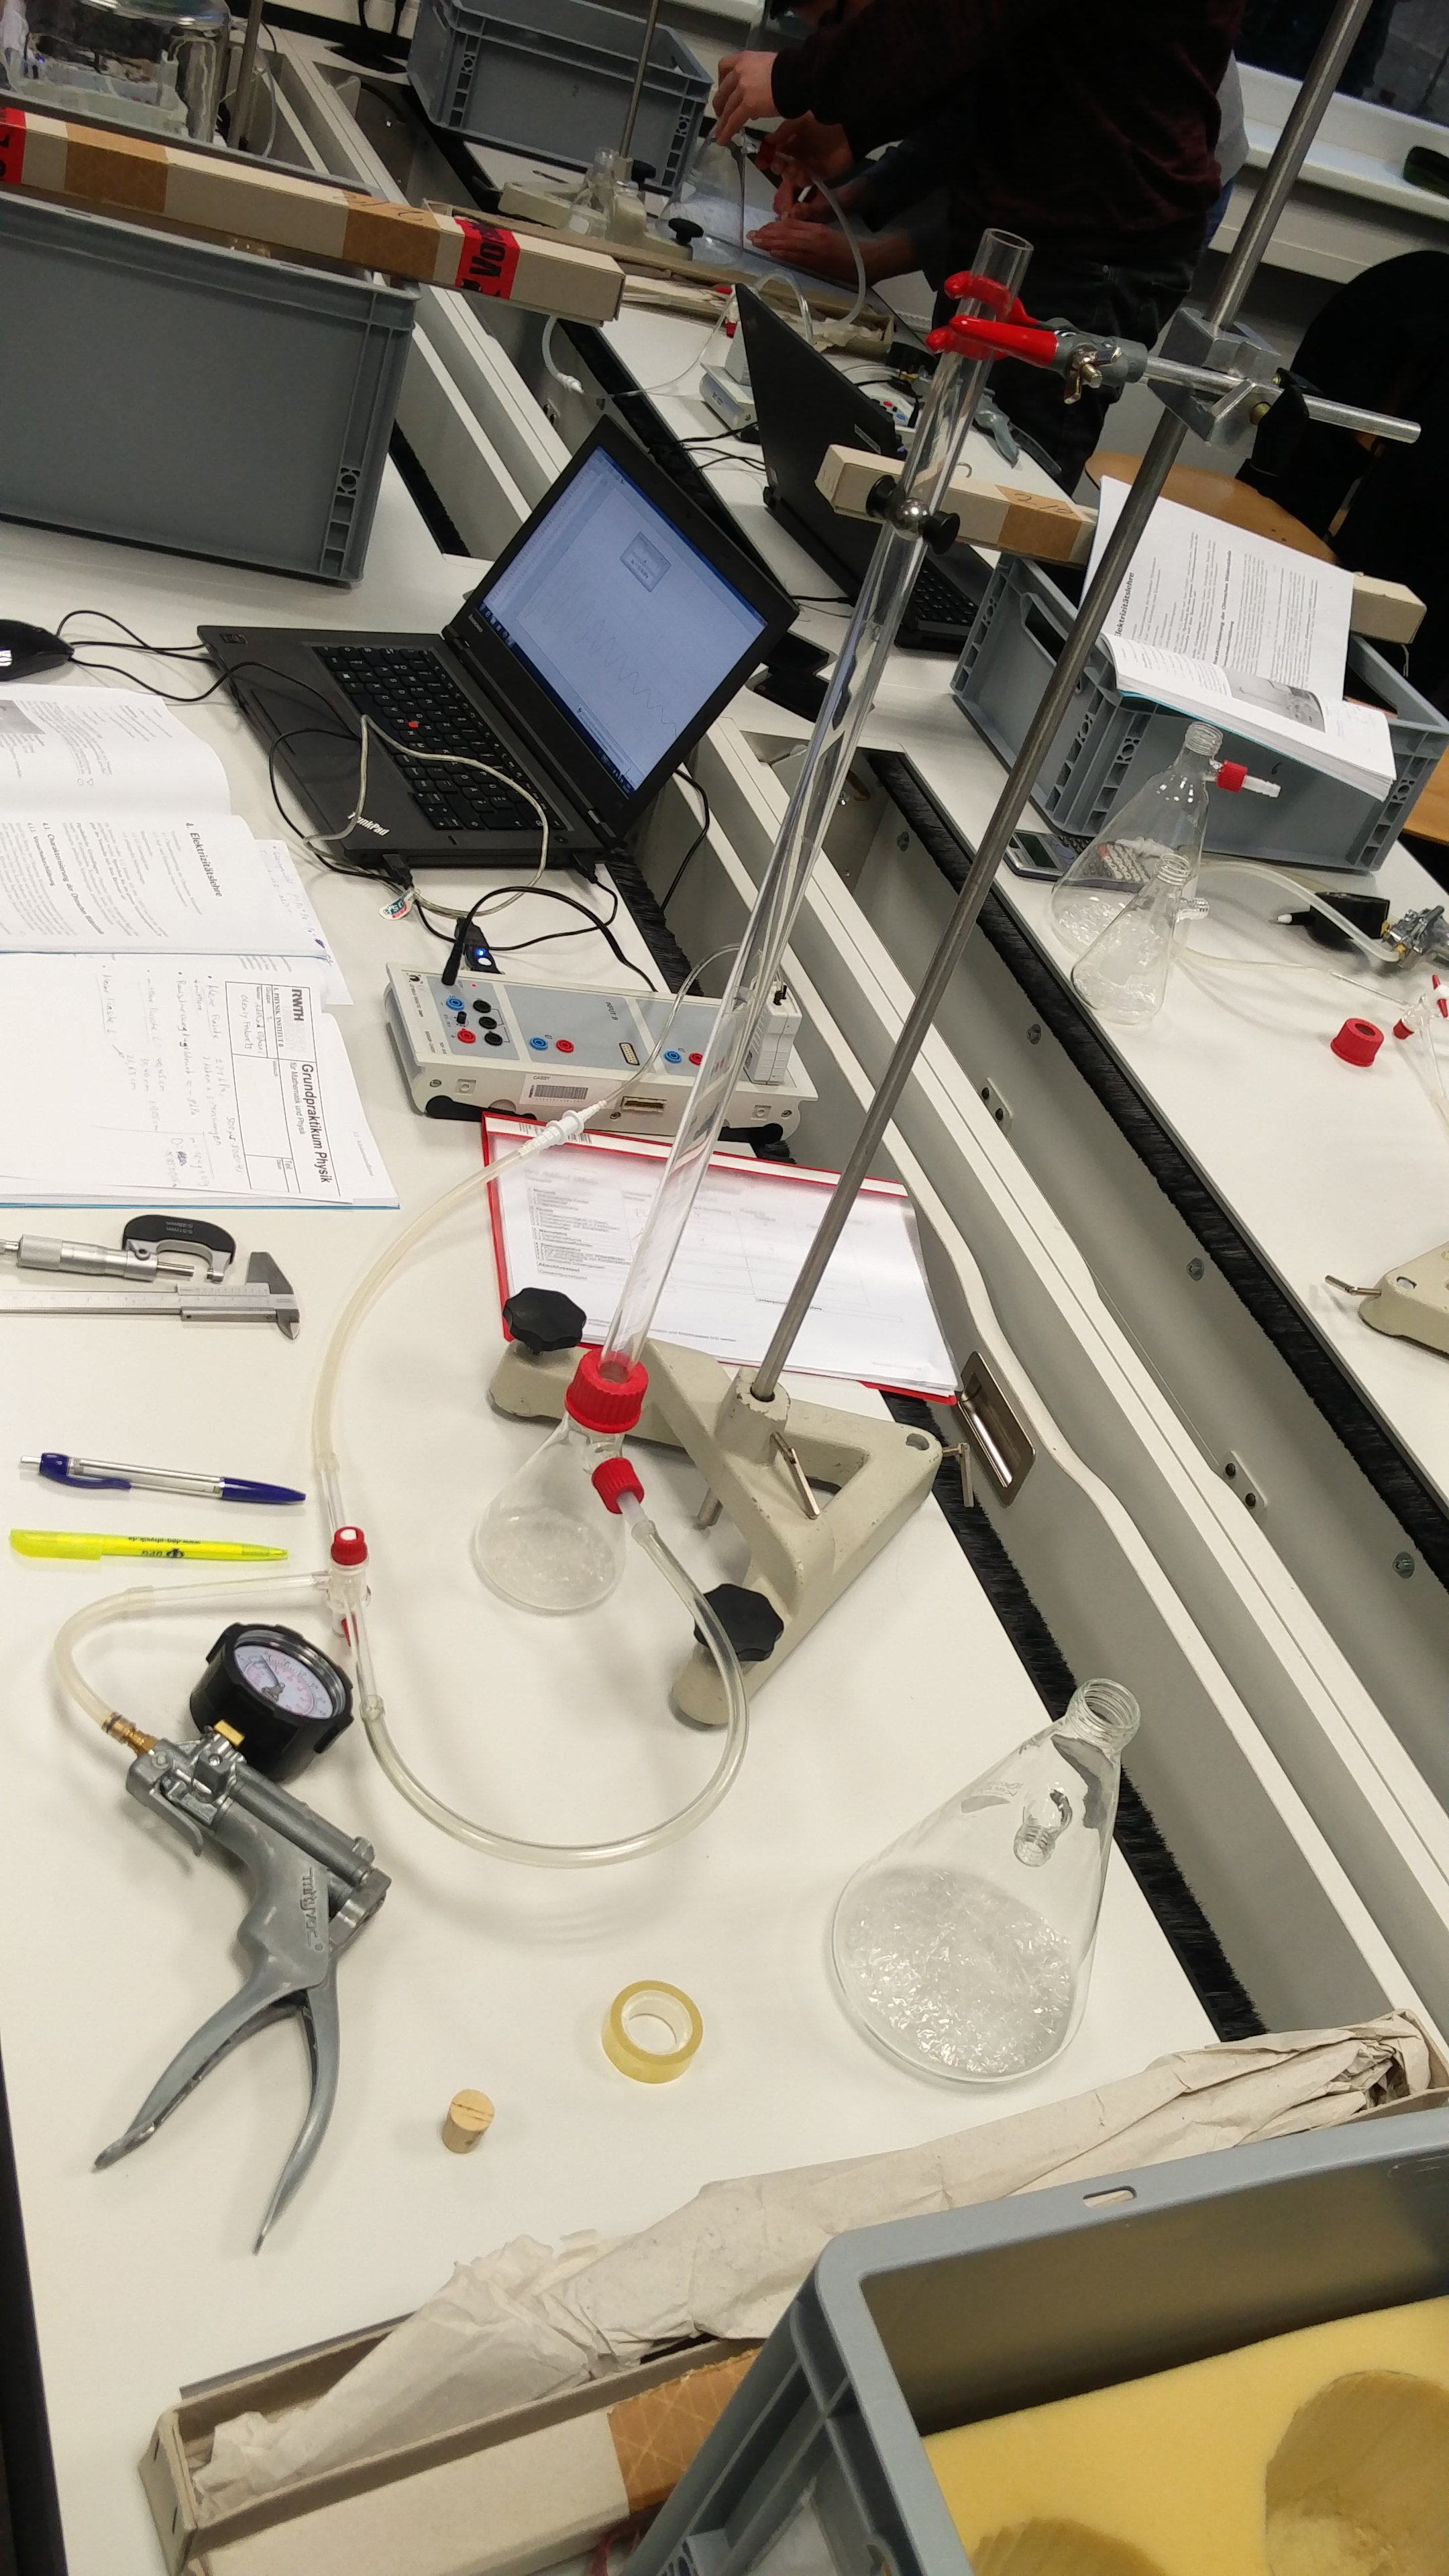
\includegraphics[scale=0.1,clip,trim=0cm 10cm 0cm 10cm]{Aufbau.jpg}
	\end{minipage}
	\label{fig:Aufbau des Versuchs}
	\caption{Aufbau und Skizze des Versuchs}	
\end{figure}



\clearpage
\section{Auswertung}
\subsection{Eckdaten der Flaschen}
Die Masse der Stahlkugel wird mit einer Waage bestimmt. Der Wert liegt bei
\begin{equation}
m = 16,4 \pm 0,1 \,g.
\end{equation}
Den Durchmesser der Kugel und des Rohres bestimmt man mit einer Mikrometerschraube, wobei sich beide zu
\begin{equation}
15,95 \pm 0,05 \,mm
\end{equation}
ergeben. Um das Volumen zu bestimmen werden zunächst die Mariottschen Flaschen leer gewogen und dann mit Wasser befüllt. Aus der Massendifferenz ergibt sich dann mit der Dichte des Wasser bei $20^\circ C$ von $\rho_W = 0.998 \; g/cm^3$ das Volumen der Flaschen. Das Volumen der großen Flasche war allerdings bereits mit vernachlässigtem Fehler angegeben. Über die Gleichung
\begin{equation}
V = \frac{m_w}{\rho_w} + \pi \frac{D^2}{4} h
\end{equation}
lässt sich das Volumen bestimmen, wobei sich der Fehler zu
\begin{equation}
\sigma_V = \sqrt{\sigma_{m_w}^2 + \left(\left(2 \frac{\sigma_D}{D}\right)^2 + \left(\frac{\sigma_h}{h}\right)^2\right) \cdot \left(\pi \frac{D^2}{4} h\right)^2}
\end{equation}
ergibt. Dabei betragen $\sigma_{m_w} = 0.1g, \sigma_D = 0.05mm, \sigma_h = 0.05cm$.


\begin{table}[H]
	\centering
	\renewcommand{\arraystretch}{1.5}
	\begin{tabular}{|c|c|c|}
		\hline Flasche & Höhen $\pm 0.05\,$[cm] & Volumen $[\cdot 10^{-6} m^3]$  \\
		\hline
		\multirow{3}{*}{\makecell{klein \\ $m_w = 317.0g$}}
				& $40.45$ & $398.46 \pm 0.52$ \\
				& $30.40$ & $378.38 \pm 0.39$ \\
				& $22.65$ & $362.89 \pm 0.27$ \\
		\hline
		\multirow{3}{*}{\makecell{mittel \\ $m_w = 1136.0g$}} 
				& $40.45$ & $1219.10 \pm 0.52$ \\
				& $30.40$ & $1199.02 \pm 0.39$ \\
				& $22.65$ & $1183.53 \pm 0.27$ \\
		\hline
		\multirow{2}{*}{\makecell{groß \\ $V = 11.315\,l$}} 
				& $42.9$ & $11400.72 \pm 0.55$ \\
				& $25.1$ & $11365.15 \pm 0.33$ \\
		\hline
	\end{tabular}
	\caption{Messdaten der verwendeten Glasflaschen}
	\label{table:Flaschen}
\end{table}

\subsection{Bestimmung der Dämpfung}
Zur Bestimmung der Dämpfung wurde mit Hilfe einer Fit-Funktion in Cassy-Lab eine abfallende e-Funktion als Einhüllende an die Schwingung angepasst.
\begin{equation}
	f(x) = A \cdot e^{-\delta t} + const
\end{equation} 
Die Parameter $A, \delta$ werden direkt ausgegeben.
Dies wird Beispielhaft je ein Mal für jede Flasche durchgeführt. Der Vergleich der Dämpfung mit der Eigenfrequenz ist in Tabelle \ref{table:Dämpfungen} zu sehen.

\begin{table}[H]
	\centering
	\renewcommand{\arraystretch}{1.2}
	\begin{tabular}{|c|c|c|}
		\hline Flasche & Dämpfung [Hz] & $\omega_0 [Hz]$ \\
		\hline 
		klein & $1.15$ & $28.08$ \\
		mittel & $0.63$ & $16.14$ \\
		gross & $0.55$ & $5.25$ \\
		\hline
	\end{tabular}
	\caption{Dämpfungen im Vergleich zur gemessenen Frequenz}
	\label{table:Dämpfungen}
\end{table}
Zu sehen ist, dass die Dämpfung vernachlässigbar klein ist (man beachte, dass diese quadratisch eingeht, siehe Gleichung \ref{eq:omega}).

\subsection{Leckmessung}
Aufgrund von Undichtigkeiten an den Verbindungsstücken der Schläuche und nach oben aus dem Rohr entweichenden Luft ist die Kugel auch ohne Auslenkung von alleine nach unten abgesunken. Daher befand sie sich nach der Schwingung nicht mehr an der selben Höhe (in der selben Gleichgewichtslage). Dies führt zu einer stetigen Änderung des Volumens während der Messung. Um diesen Effekt abzuschätzen wurde bei jeder Flasche eine Leckmessung durchgeführt, wobei die Zeit gestoppt wurde die die Kugel benötigte, um von einer Höhe von $50$cm auf $30$cm abzusinken. Die Ergebnisse sind in Tabelle \ref{table:Leckmessung} zu sehen.

\begin{table}[H]
\centering
\renewcommand{\arraystretch}{1.2}
\begin{tabular}{|c|c|c|}
	\hline Flasche & Strecke[cm] & Zeit[s] \\
	\hline klein & $20$ & $30,25$ \\
	mittel & $20$ & $33,03$ \\
	groß & $20$ & $28,12$ \\
	\hline
\end{tabular}
\label{table:Leckmessung}
\caption{Leckmessung}
\end{table}

Daraus ergibt sich eine Absinkgeschwindigkeit von $\approx 0.6$ cm/s, was bei einer Messzeit von 4s eine Volumenänderung von $\approx 5cm^3$ ergibt. Es ist ersichtlich, dass dies bezogen auf die Volumen in Tabelle \ref{table:Flaschen} keinen großen Einfluss hat.


\subsection{Bestimmung der Frequenzen}
Im Folgenden sind Beispielhaft die Rohdaten jeweils einer Schwingung bei den drei Flaschen zu sehen. Es ist zu erkennen, dass bei der großen Flasche viel weniger Perioden aufgetreten sind, als bei den kleineren Flaschen.

\begin{figure}[H]
	\centering
	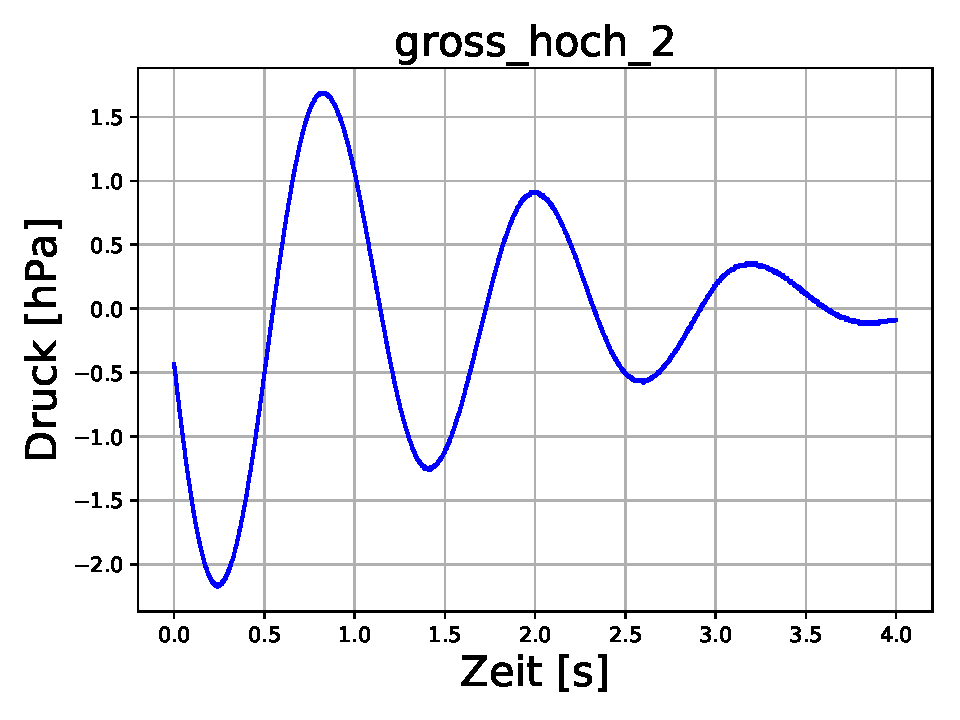
\includegraphics[scale=0.4]{../Plots/gross_hoch_2.pdf}
	\caption{Druckverlauf bei der großen Flasche bei hoher Position}
\end{figure}

\begin{figure}[H]
	\centering
	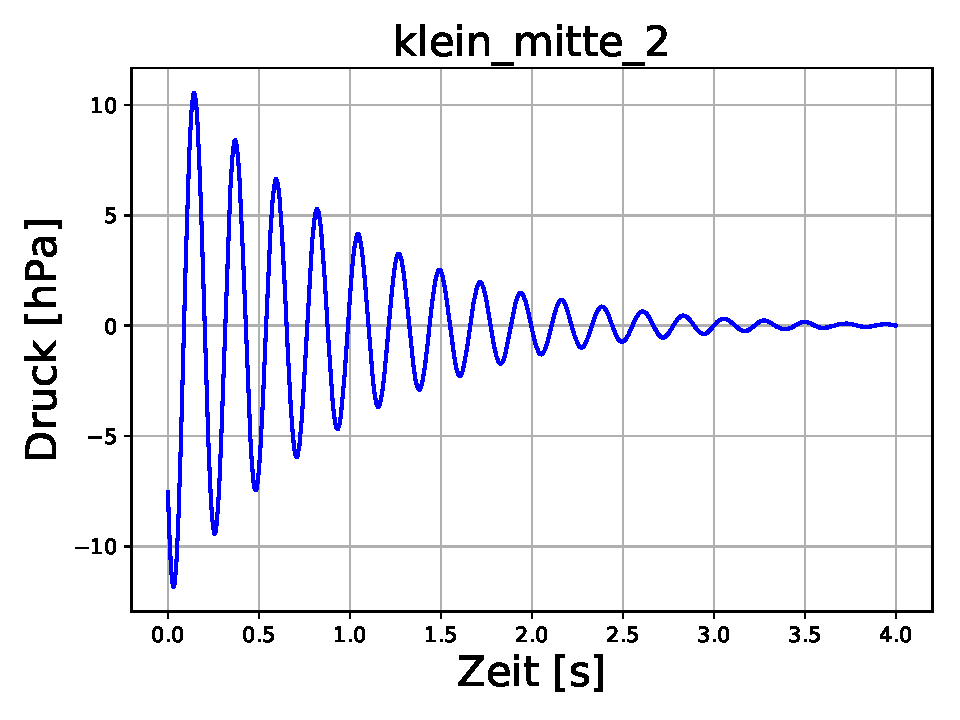
\includegraphics[scale=0.4]{../Plots/klein_mitte_2.pdf}
	\caption{Druckverlauf bei der kleinen Flasche bei mittlerer Position}
\end{figure}

\begin{figure}[H]
	\centering
	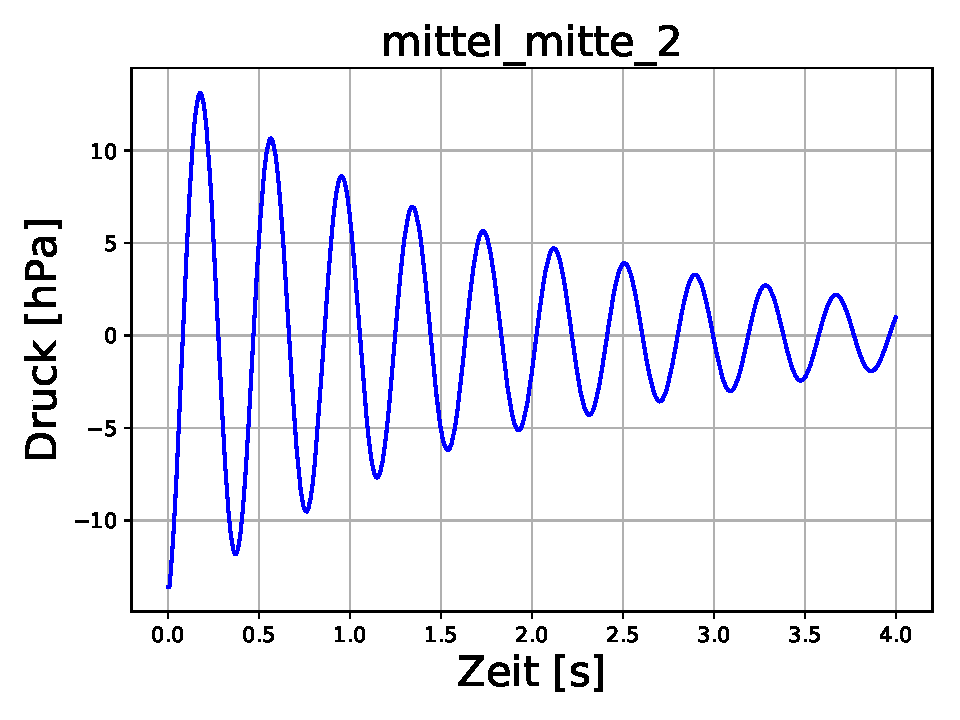
\includegraphics[scale=0.4]{../Plots/mittel_mitte_2.pdf}
	\caption{Druckverlauf bei der mittleren Flasche bei mittlerer Position}
\end{figure}

Um die Frequenz der Schwingungen zu bestimmen, wurden mit Hilfe von CASSY-Lab die Nulldurchgänge mit entsprechende Zeiten $t_1,t_2$ bestimmt und die entsprechende Periodenanzahl $n$ gezählt. Daraus kann dann mit Hilfe der folgenden Formeln die Eigenfrequenz bestimmt werden.
\begin{equation}
T = \frac{t_2 - t_1}{n} \quad \omega = \frac{2\pi}{T} \qquad \sigma_\omega = \omega \cdot \frac{\sqrt{2} \cdot \sigma_t }{n} \cdot \frac{2\pi}{T^2}
\end{equation}
Wobei hier $\sigma_t = 0.5 ms$ die Genauigkeit der Bestimmung eines Nulldurchgangs ist, die hier dem Messintervall entspricht.

Da die Schwingung pro Position immer jeweils 3 Mal aufgezeichnet wurde, wurden diese Werte jeweils gemittelt und der Fehler auf den Mittelwert bestimmt. 

Die Bestimmung der Frequenz über eine Fouriertransformation erwies sich als zu ungenau, da die Abstände zwischen zwei Punkten im Frequenzspektrum bedingt durch die Dauer der Aufzeichnung $1/4s$ betrugen. Hierfür müsste man entweder länger ein Rauschen messen oder Nullen an die Daten anhängen.

\subsection{Bestimmung von $\kappa$}
Der Außendruck $p_0$ wurde zum Zeitpunkt des Versuchs von der Wetterstation RWTH-Hörn zu $977 \,hPa$ abgelesen. Zur Bestimmung des Gesamtdrucks wird zusätzlich noch eine Messung des Drucks durch die Gewichtskraft der Kugel über $8s$ gemacht. Dabei ergibt sich durch Bildung des Mittelwerts
\begin{equation}
p-p_0 = \frac{m g}{A} = 7.95 \pm 5 \cdot 10^{-4} \, hPa
\end{equation}

Um den Adiabtenkoeffizienten zu bestimmen wird $\omega^2$ über $1/V$ aufgetragen und eine Ausgleichsgerade an die Messpunkte gelegt.
Bei dieser Auftragung müssen auch die veränderten Fehler auf den Kehrwert des Volumens und auf $\omega^2$ berücksichtigt werden:
\begin{equation}
\sigma_{1/V} = \frac{\sigma_V}{V^2} \qquad \sigma_{\omega^2} = 2 \omega \cdot \sigma_{\omega}
\end{equation}
Aus der Steigung $a$ kann man nun $\kappa$ bestimmen
\begin{equation}
\kappa = \frac{a m}{p A^2},
\end{equation}
Der Fehler auf die Fläche stammt hierbei aus der Messung des Durchmessers:
\begin{equation}
\sigma_A = 2 \cdot \frac{\sigma_D}{D} \cdot A
\end{equation}
Der Fehler auf Kappa lautet dann mit dem Gaußschen Fehlerfortpflanzungsgesetz
\begin{equation}
\sigma_{\kappa} = \kappa \cdot \sqrt{\left(\frac{\sigma_a}{a}\right)^2 + \left(\frac{\sigma_m}{m}\right)^2 + \left(\frac{\sigma_p}{p}\right)^2 + 4 \left(\frac{\sigma_A}{A}\right)^2}
\end{equation}
Dabei ergibt sich der Fehler auf den Druck nur aus dem Mittelwert des Schweredrucks, da der Außendruck $p_0$ ohne Fehler angegeben war. Daher haben dieser und der Fehler auf die Masse keine große Auswirkung auf den Gesamtfehler.
Die lineare Regression zur Bestimmung von $\kappa$ ist in Abbildung \ref{fig:Linregress} zu sehen. Dabei fällt auf, dass die Frequenz der Schwingung an der hohen Position in der kleinen Flasche im Gegensatz zu den anderen heraussticht.

\begin{figure}[H]
	\centering
	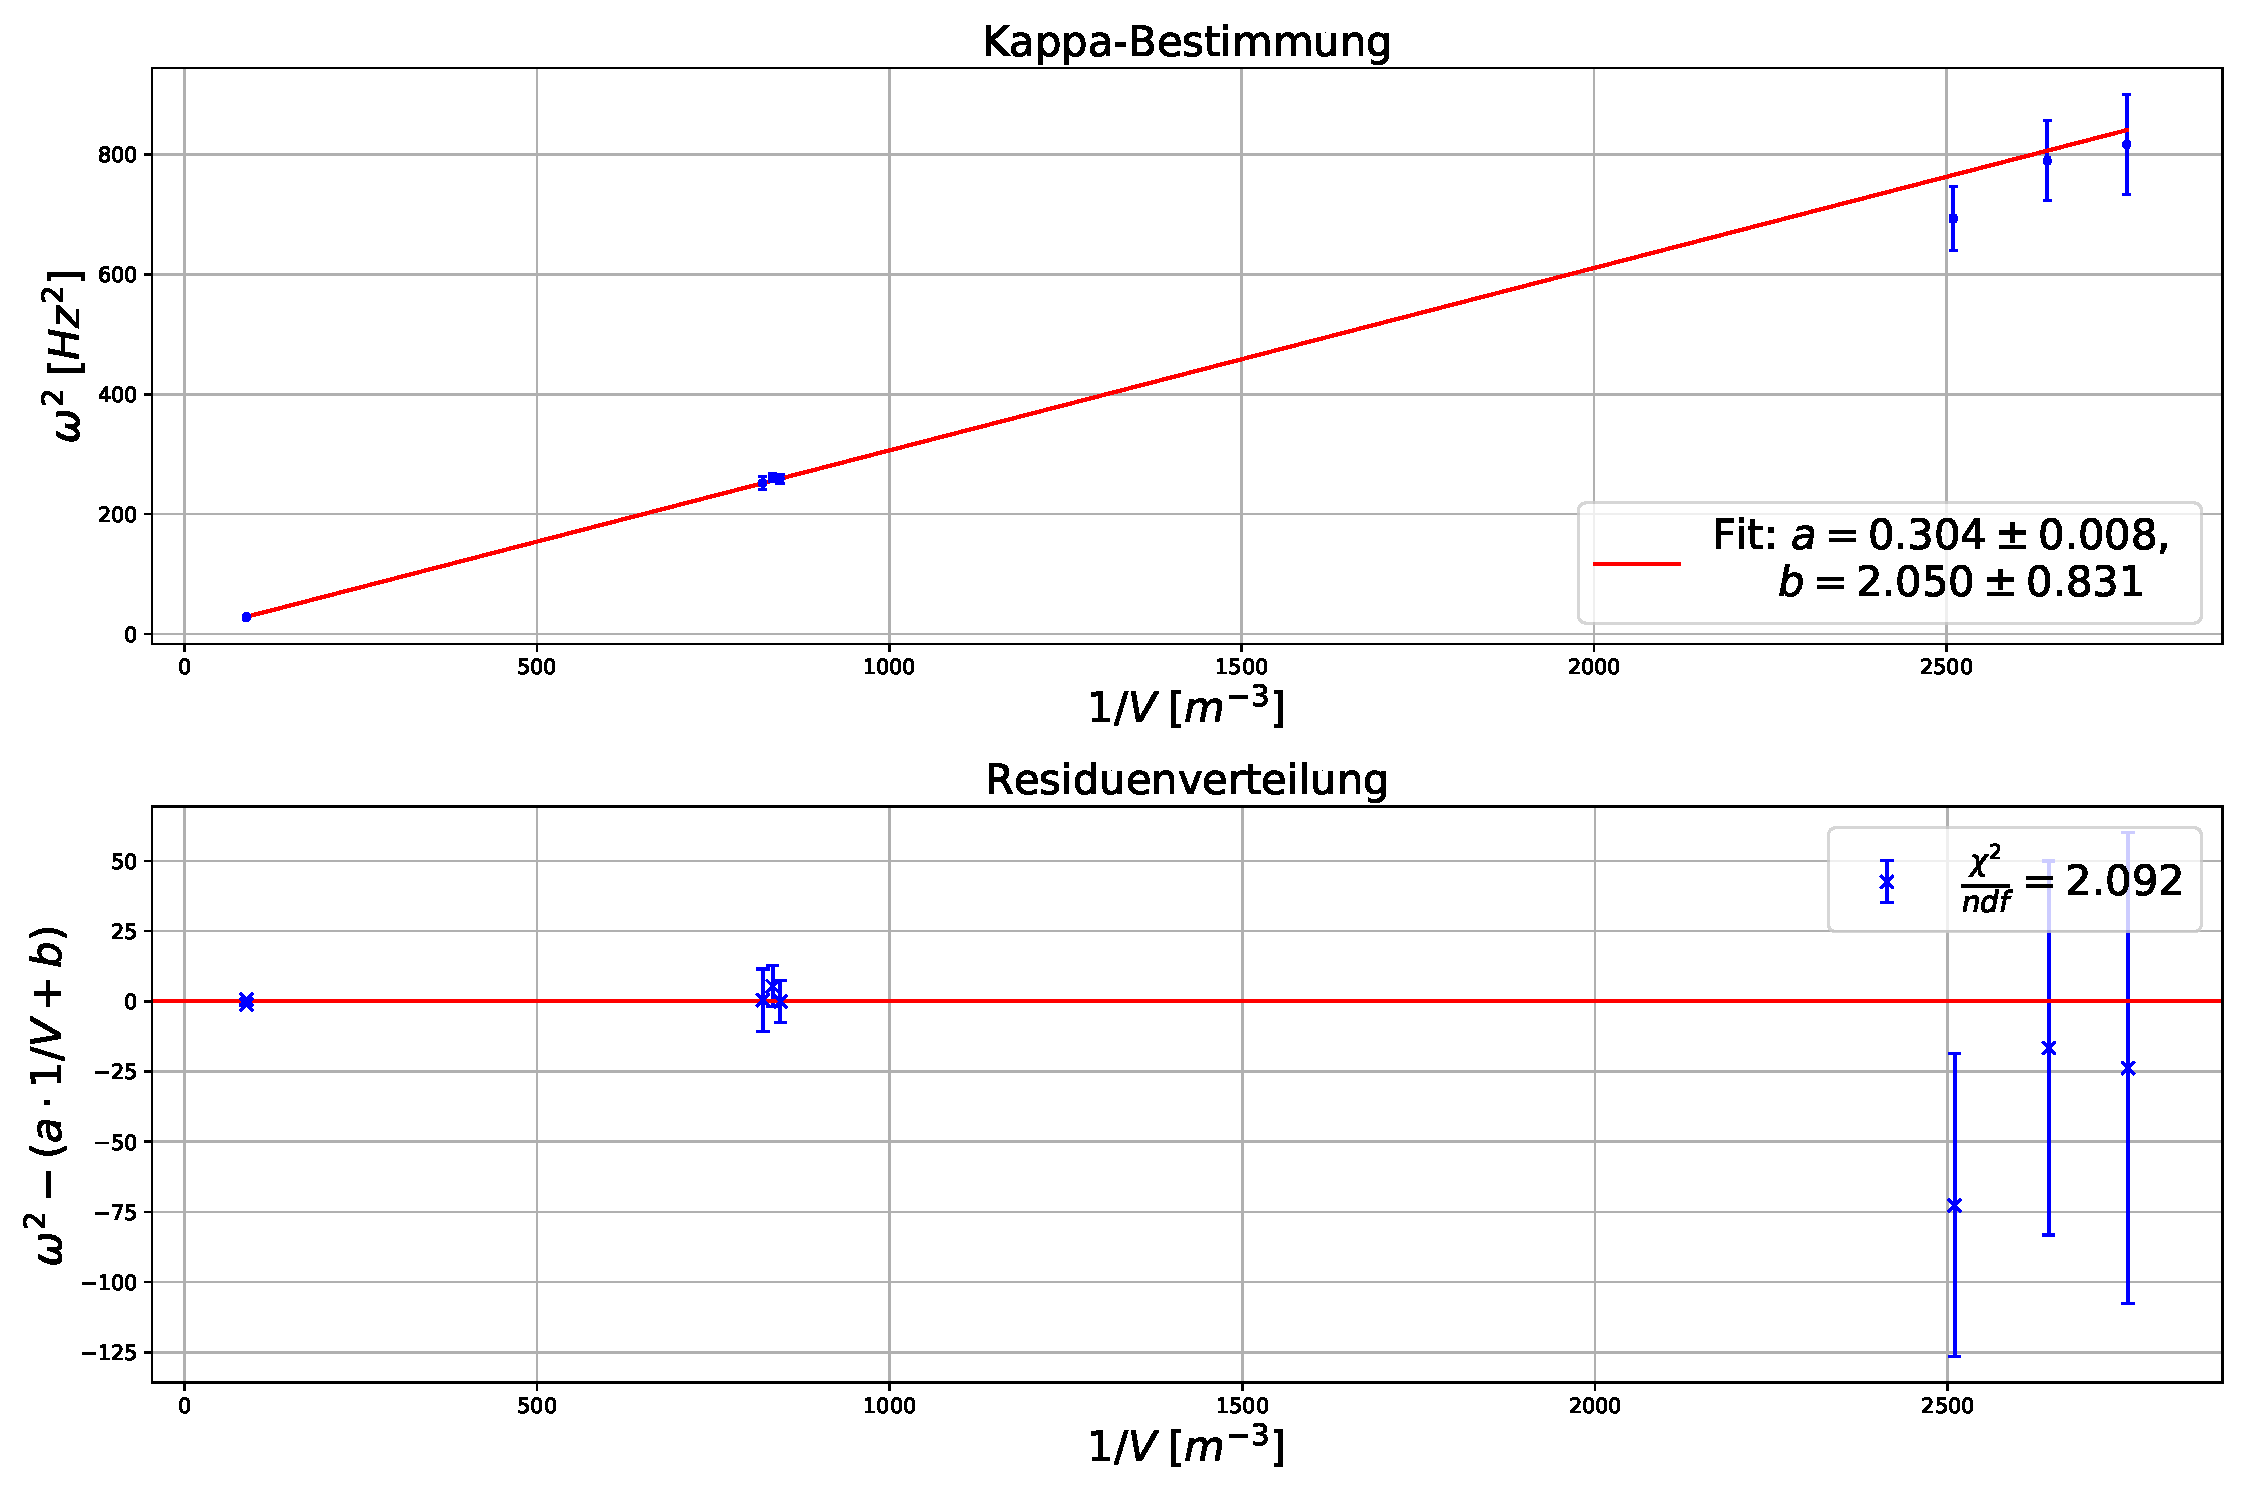
\includegraphics[scale=0.4]{../Plots/Kappa-Bestimmung_mitWert_NEU.pdf}
	\caption{Bestimmung von Kappa mit ihrer Residuenverteilung ohne Auslassung eines Wertes}
	\label{fig:Linregress}
\end{figure}

Daher haben wir diesen Wert rausgelassen und die Auswertung nochmal durchgeführt. Das Ergebnis ist in \ref{fig:LinregressOhneWert} zu sehen.

\begin{figure}[H]
	\centering
	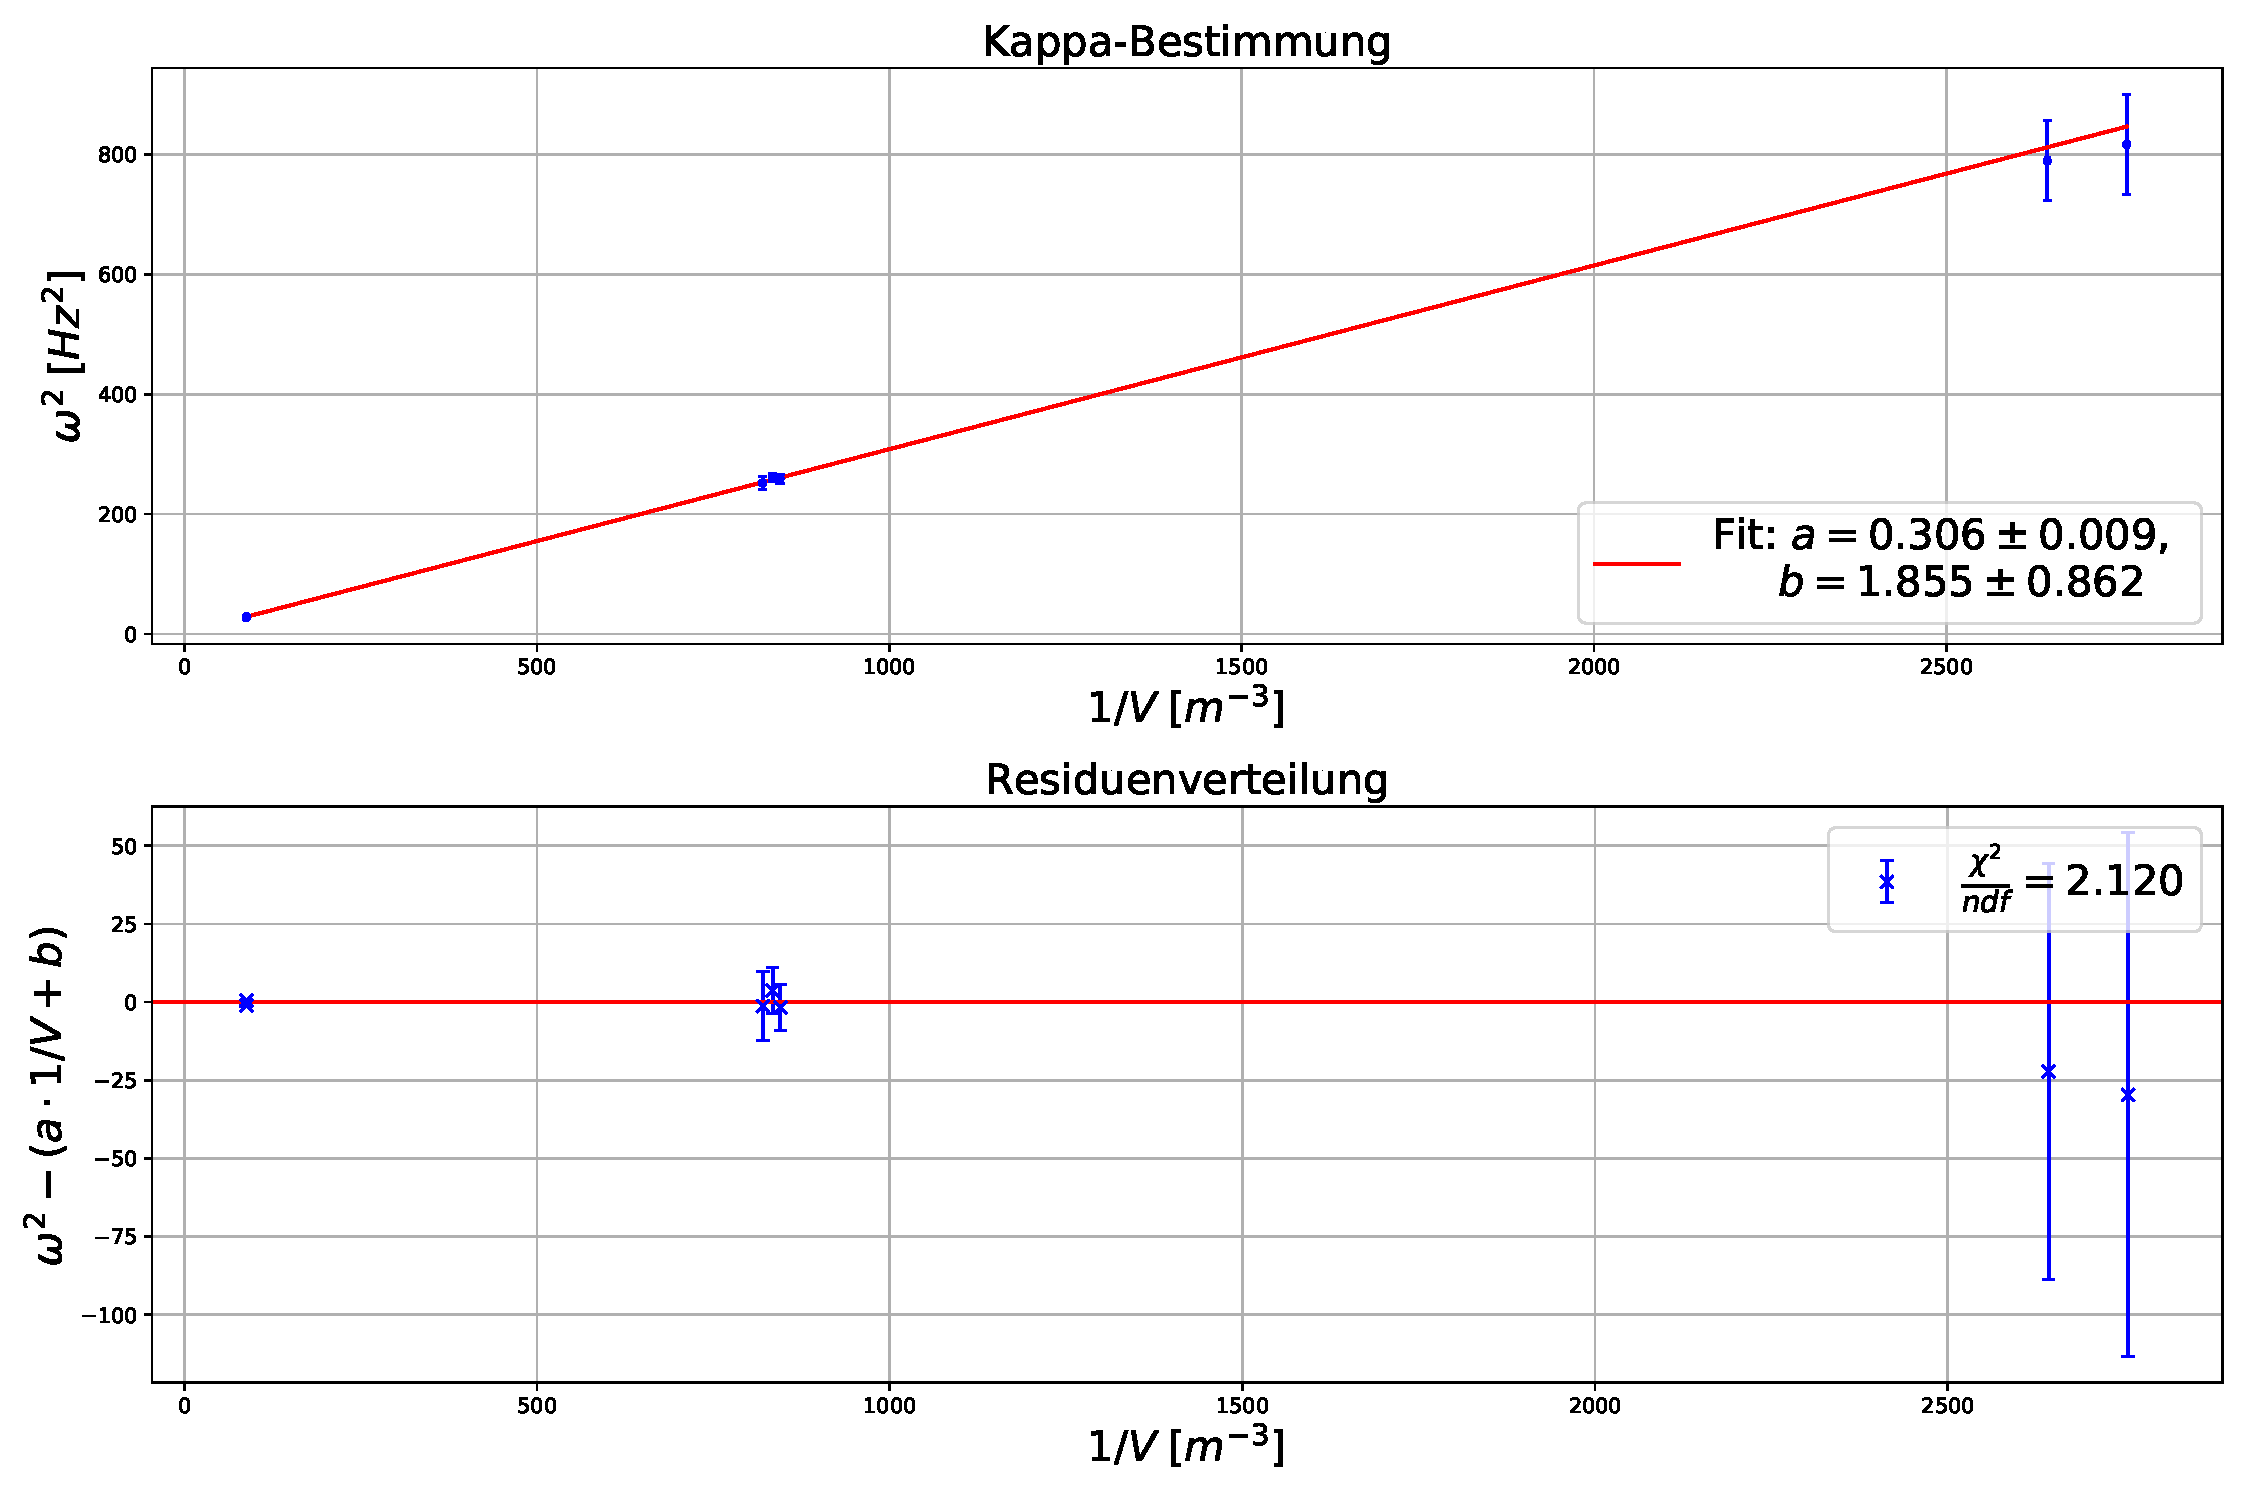
\includegraphics[scale=0.4]{../Plots/Kappa-Bestimmung_ohneWert_NEU.pdf}
	\caption{Bestimmung von Kappa mit ihrer Residuenverteilung mit Auslassung eines Wertes}
	\label{fig:LinregressOhneWert}
\end{figure}

Durch eine starke Abweichung der Volumen der Flaschen zueinander ist die Gruppierung der Messwerte im Plot zu erkennen. Aufgrund dieser Volumenunterschiede sind auch die kombinierten Fehler auf die Messwerte der drei Flaschen deutlich unterschiedlich, bei der kleinsten Flasche entsprechend am größten. Außerdem liegen die Werte der kleinen Flasche immernoch unter der Geraden, aber mit Ihren Fehlerbalken darauf. Das $\chi^2/ndf$ liegt mit einem Wert von $2.1$ in der Nähe vom erwarteten Wert 1. 
Damit ist unser Ergebnis auf Kappa
\begin{equation}
\kappa = 1,287 \pm 0,042
\end{equation}
Dieser Wert liegt in einer $2.7 \, \sigma$-Umgebung vom wahren Wert von $\kappa = 1.4$.


\section{Fazit}
Die Versuche mit der kleinen und der mittleren Flasche haben gut funktioniert. Bei der großen Flasche war es schwer die Kugel zum schwingen zu bringen, ohne dass die Stahlkugel beim Auslenken aus der oberen oder unteren Öffnung rausflog. Aufgrund dieser Begrenzung in der Amplitude ließen sich auch nur wenige Perioden aufzeichen.

Durch die großen Unterschiede der Volumen der Flaschen waren die Messwerte der Flaschen in drei 'Wolken' lokalisiert. Im Residuenplot sind deutliche Unterschiede der Fehler zu erkennen. Dennoch hat die lineare Regression gut funktioniert. Der bestimmte Wert des Adiabatenkoeffizienten lag noch in einer $3 \,\sigma$-Umgebung.

Eine nicht berücksichtigte Fehlerquelle auf das Volumen sind zum Beispiel die Schläuche im Versuchsaufbau, die auch zum Gesamtvolumen beitragen. Womöglich kann dies zur Abweichung im Wert von $\kappa$ geführt haben. Die Dämpfung und die Entweichung der Luft haben sich allerdings als vernachlässigbar erwiesen.

Außerdem ist auch die Annahme eines adiabatischen Prozesses eine Idealisierung und in der Praxis nie zu 100\% gegeben, was auch zu der Abweichung von $\kappa$ führen könnte.






\listoffigures
\listoftables


\end{document}

